\documentclass[11pt,reqno]{amsart}

\setlength{\textheight}{8.8in}
\setlength{\topmargin}{-.1in}
%\setlength{\textwidth}{6in}
%\setlength{\oddsidemargin}{.26in}
%\setlength{\evensidemargin}{.26in}
\parskip=.08in

\usepackage[pagebackref]{hyperref} % for pdflatex
%\usepackage[hypertex,pagebackref]{hyperref} % for latex
\usepackage{xcolor}
\usepackage{amsmath,amsthm}
\usepackage{amssymb}
\usepackage{graphicx}
\usepackage[mathscr]{eucal}
\usepackage{MnSymbol}
\usepackage[frame,ps,matrix,arrow,curve,rotate,all,2cell,tips]{xy}
\usepackage{enumerate}


\setcounter{tocdepth}{1}

% The second argument here is about how to label the theorems, e.g. Theorem 2.2 is the second thing in section 2. The first thing in section 2 is subsection 2.1.
\newtheorem{theorem}[subsection]{Theorem}
\newtheorem{lemma}[subsection]{Lemma}
\newtheorem{sublemma}[subsection]{Sub-Lemma}
\newtheorem{proposition}[subsection]{Proposition}
\newtheorem{corollary}[subsection]{Corollary}
\newtheorem{thm}[subsection]{Theorem}
\newtheorem{prop}[subsection]{Proposition}



%%% The following environments have roman body.

\theoremstyle{definition}
\newtheorem{definition}[subsection]{Definition}
\newtheorem{example}[subsection]{Example}
\newtheorem{remark}[subsection]{Remark}
\newtheorem{assumption}[subsection]{Assumption}
\newtheorem{convention}[subsection]{Convention}
\newtheorem{notation}[subsection]{Notation}
\newtheorem{conjecture}[subsection]{Conjecture}
\newtheorem{construction}[subsection]{Construction}
\newtheorem{work}[subsection]{Just For Us}

\numberwithin{equation}{subsection}

%\newtheorem{defn}[subsubsection]{Definition}
% donald has this command reserved
\newtheorem{conj}[subsection]{Conjecture}
\newtheorem{fact}[subsection]{Fact}
\newtheorem{problem}[subsection]{Problem}

% Common number systems
\renewcommand{\P}{\mathbb{P}}
\newcommand{\N}{\mathbb{N}}
\newcommand{\bbP}{\mathbb{P}}
\renewcommand{\H}{\mathbb{H}}

\newcommand{\Q}{\mathbb{Q}}
\newcommand{\R}{\mathbb{R}}
\newcommand{\Z}{\mathbb{Z}}
\newcommand{\F}{\mathbb{F}}

\renewcommand{\O}{\mathsf{O}}
\newcommand{\bbA}{\mathbb{A}}
\newcommand{\bbC}{\mathbb{C}}
\newcommand{\bbG}{\mathbb{G}} % Additive/Multiplicative group
\newcommand{\G}{\mathbb{G}} % Additive/Multiplicative group

%\newcommand{\balpha}{\mathbb{\upalpha}}
%\newcommand{\bmu}{\mathbb{\upmu}}









\newcommand\tab[1][1cm]{\hspace*{#1}}

\begin{document}



\title[CS/MATH 335 Final Paper] {Recommendation Systems \\ By: Matt Iammarino and Taylor Heilman\\ }
\maketitle





\tableofcontents

\section{Introduction}

\tab  The use of \textit{Recommender Systems} has vastly grown in the past decade due to the explosion of online retail as well as streaming services such as Pandora and Netflix. With 90\% of Netflix streams and 35\% of Amazon's revenue reportedly coming from recommendations, having a highly efficient recommendation system is a necessity for web-based companies in 2016 and thus are becoming more and more integrated into our everyday lives. Essentially, a Recommendation System ideally provides recommendations of items, ranging from songs, movies, products, etc., to a user using data obtained from either the said user or from other users exhibiting similar trends as the user in question. This paper combines several scholarly sources in order to stream-line the subject of Recommender Systems in a succinct fashion for the reader. Because of this, the information presented is a simple overview of the advanced topic that is Recommendation Systems. The topics covered include Utility Matrices, Content-Based Systems, Collaborative Filtering, as well as several algorithms used in each system. It is worthy to note that the knowledge of intermediate computer science topics is necessary, as this paper is aimed toward undergraduate computer science students.
\newline

\section{Modeling Recommender Systems with a Matrix}
\tab Recommender Systems use what is called a Utility Matrix in order to help determine recommendations for various subjects. The Utility Matrix takes into account both users and items in order to try to correlate values between a user and an item. A user can be anywhere from a single person to a company and the items can be any type of item that can be used for recommendation. The Utility Matrix will have users along the rows and then items along the columns. Each user will have many columns associated with it regarding different items among many different disciplines. For each entry within the matrix, the corresponding value represents some sort of preference level that the user had for the specific item. This preference can be as simple as a rating out of five stars or more complicated preferences such as a specific characteristic about the item that helps to categorize it. An easy example would be users and there ratings for certain movies. An example for a utility matrix representing this scenario could look like this:
\newline
\[
M=
  \begin{bmatrix}
    3 &  & 1 &  & 2 & & 5 \\
    1 & 2 & & 3 & 1 & &\\
    & 1 & & 2 & 1 & 4 &\\
     & 1 &  & 4 &  & & 5 \\
  \end{bmatrix}
\]
\newline
Within this matrix, each row would be a different user and each column would be a different movie. Notice that each user has ratings for a given movie out of 5. From this matrix we can conclude some facts such as the last movie, column five, was rated 5 out of 5 by both users one and 4 and the third movie, column three, may not be very good based upon the one out of 5 rating from user one. As you may notice, this utility matrix is sparse, meaning there are blanks within the matrix. This means not every user has a rating for each of the movies presented.This is the case for most utility matrices for recommender systems. A main reason for the sparseness comes from the fact that the only way to obtain a rating for the matrix is to obtain feedback for a user. Often times users  refrain from rating a movie title after viewing it because they feel like it's a waste of time.  Another issue is many users will only leave a rating if the movie was extremely good or on the other hand extremely bad, meaning most rating in the matrix are either 1's or 5's. Therefore, the ultimate goal of a recommender system is to try to predict those blanks as accurately as possible. By predicting the blanks, a system then can be able to give recommendations to users based upon high-predicted rankings. Predicting the blanks can cause a challenge for systems to do, especially if the matrix is very sparse. These predictions need to be as accurate as possible in order to ensure valid recommendations. There are a few different methods for predicting these blanks and they have to do with the type of architecture behind the systems. For this paper, we focus on two different types of architecture: Content-Based and Collaborative Filtering.

\section{Content-Based Systems}

\tab Content-Based Systems are recommender systems that specifically focus on the distinct properties of the items within the matrix. From the properties, certain measurements can be made to try to measure the similarity between different items within the matrix. The similarities then can help make recommendations for different users. The main goal for a content-based system is to try to construct profiles for both the users and the items in order to calculate the similarities between the profiles and then further provide a recommendation. The first profile constructed is an item profile. An easy example to show is a profile for a movie. For example, let's look at the 2015 Star Wars movie, \textit{Episode VII the Force Awakens}. The profile may look something like this:

\begin{center}
\fbox{\begin{minipage}{15em}
Director: J. J Abrams \newline

Genre: Action and Adventure\newline

Actors: Harrison Ford, Mark Hamill, Carrie Fisher, Adam Driver, Daisy Ridley, John Boyega, etc. \newline

Year: 2016 \newline
\end{minipage}}
\end{center}


Similarly, profiles need to be created for users. The user profiles will correspond to the same properties that were used to construct the item profiles which will allow the system to discover the specific properties a user rated highly. For example, if a user consistently  rates movies starring Leonardo Dicaprio highly, then their profile would show the high rating for Leonardo Dicaprio and the system would likely recommend other movies starring Leonardo Dicaprio.\newline



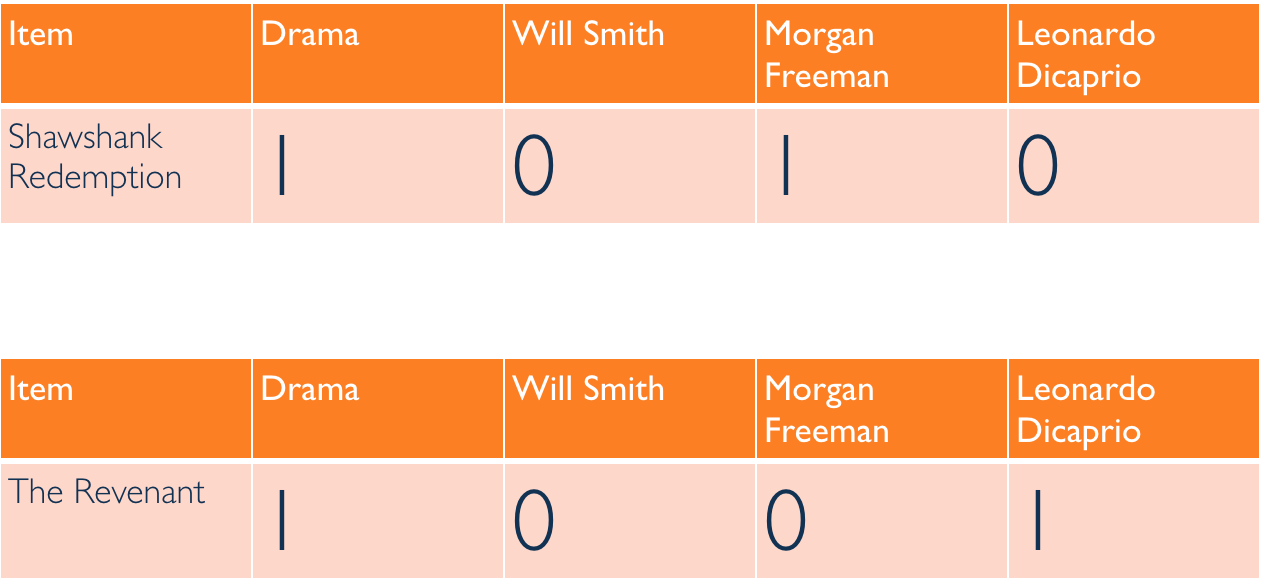
\includegraphics[width=\textwidth]{pic2}


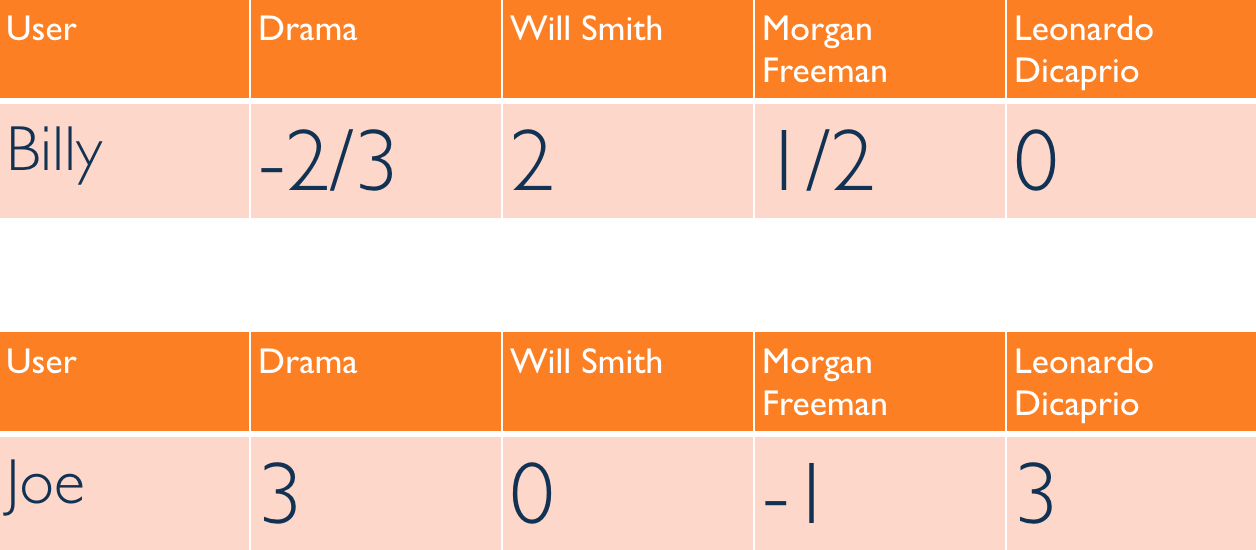
\includegraphics[width=\textwidth]{pic3}

These are examples of both User and Item profiles using boolean variables. In the Item profiles, there is a 1 in the profile if that characteristic is a property of the item, for example there is a 1 in the Morgan Freeman characteristic of Shawshank Redemption because Morgan Freeman is an actor in that movie, while Will Smith has a 0 because he was not in the movie. Using these same characteristics, User profiles can be created as well. The average rating is computed for a given User and the values in the characteristics of a given User are, on average, how differently they would rate an item with this characteristic from their average rating. For example, a 3 in Drama for Joe means that on average he rates items with the characteristic of Drama 3 points higher than his average. 

The ultimate goal of the Content-Based System is to directly relate the content on specific items to the content that users rated highly. The correlations between these properties will allow the system to then provide recommendations for each user. \newline

\section{Collaborative Filtering}
The second type of architecture that we will discuss is collaborative filtering. This type of recommendation relies on trying to determine how similar two users or two items are. From that, if two users are deemed to be similar, then the system can recommend items to one user that the other similar user enjoyed and vice versa. The same thing can be done for items. If two items are deemed similar, then the system can recommend an item that is similar to a previous item that a user rated highly. The biggest decision to be made within this type of system is trying to figure out the correct way to measure similarity. Some of the methods that we have found will be described later in the paper. \newline

It turns out that trying to find similar items is much easier to calculate than trying to find similar users. The problem becomes that although finding similar items can be easier to solve, determining if users are similar becomes more effective because knowing that two users are similar can give much more information about various items, where knowing two items are similar does not tell much about various users. Nevertheless, by finding these similarities, the blanks in the matrix can then be predicted from the similarities found. This will then allow systems to make accurate recommendations for the users. 
\newline

\section{Hybrid Recommender Systems}

 Now that you have an understanding of both Collaborative Filtering and Content-Based Systems we can look at Hybrid Recommender Systems.  A Hybrid Recommender System takes both Collaborative Filtering and Content-Based Systems to output more accurate recommendations.  The implementation of combining the two systems can be done in multiple ways.  A system can simply calculate the Content and Collaborative recommendations separately and then combine the two outputs.  Another option is to add collaborative-based capabilities to a content-based system, or vice versa.  And lastly, a system can simply unify both approaches into one model.
 
 
 
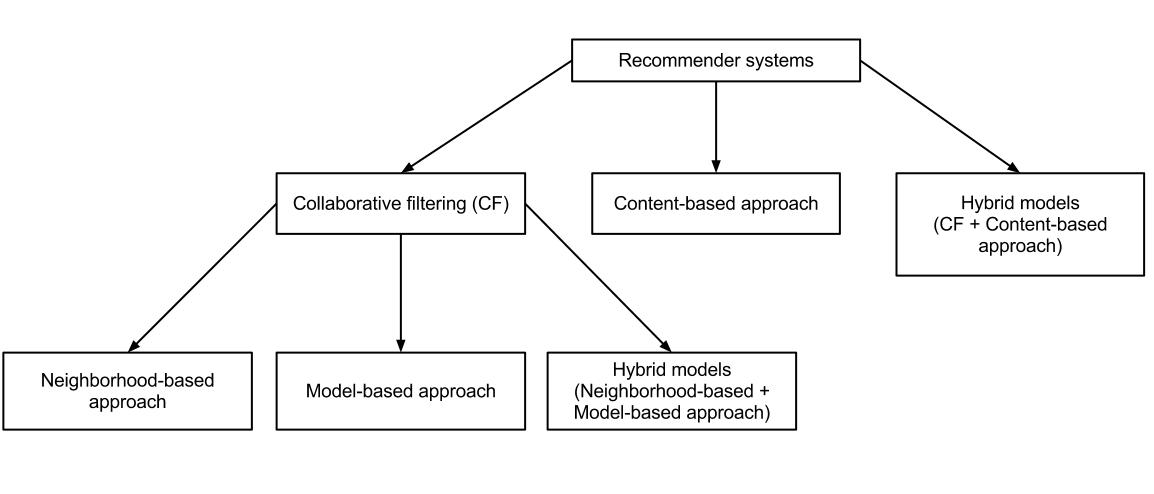
\includegraphics[width=\textwidth]{pic1.jpg}


 
 Hybrid Recommender Systems are valuable because by combining the two approaches, content and collaborative, into one singular approach common issues, such as scarcity in matrices or cold-starts, become less problematic in the Hybrid Implementation. Also, Hybrid Recommender Systems are valuable to understand because the Netflix Recommendation System is an implementation of a Hybrid System.
\newline
 
\section{Content-Based Algorithm}

Content-Based Algorithms focus specifically on the items and their properties. The main goal behind these algorithms are solely based on trying to calculate the similarity between two items or an item to a User's preferences based upon its profile.
Here, we will discuss a few of the common metrics used to conduct similarities. 

Cosine Distance - The goal of this metric is to try to compute the cosine of the angle between two vectors. In our case, the two vectors, $x$ and $y$, will both be items within the database. Calculating the similarity uses the equation

\[
	cos(x,y) =		\frac{x  \boldsymbol{\cdot} y}{\begin{Vmatrix} x \end{Vmatrix}_2 *	\begin{Vmatrix}  y\end{Vmatrix}_2}
\]
where $x$ and $y$ are both vectors and $\boldsymbol{\cdot}$ denotes the dot-product.[1]

Euclidean Distance- Another metric that can be used to try to determine how similar two vectors are is calculated by using the formula
\[
	dist([x_1, x_2,.., x_n], [y_1, y_2,..., y_n]]= \sqrt{\sum_{i=1}^{n} |x_i - y_i|^{2}}
\]
where each vector has $n$ properties for an item.[1]

Jaccard Similarity- This similarity metric tries to compute the similarity between two items by representing at item as a set of their properties. To compute the similarity we use the following formula
\[
	Similarity(X,Y) = \frac{|X \cap Y|}{|X \cup Y|}
\]
Notice that this similarity metric calculates how many properties they have similar out of the total number of properties. A value closer towards 1 will imply a higher similarity. [1]


Any of these metrics can help to figure out which items are most similar. Content-based systems focus solely on the item-data and not worrying about user ratings. From these calculations, a system can just compute items most similar to an item that a given user either bought, watched, or viewed. A good example of an content-based recommendation system is Pandora. Pandora is a online music player that streams songs to a user. A user will select a station, such as a genre, artist, or a song, and then the application will play songs that are similar to the selected station. In essence, Pandora works as a smart radio. In this scenario, the songs that Pandora plays for a specific station come from the most similar songs to either the genre, artist, or song that the user selects as its station. Also, a content-based system could find the items that are most similar to the User profile preferences that have been calculated. For example, Joe has a high drama rating and a high Leonardo Dicaprio rating, so \textit{Inception} may be a great recommendation to Joe because it has similar properties.
\newline

\section{Collaborative Filtering Algorithms}
There are a couple paths to be taken when deciding which algorithms to use when using Collaborative Filtering. The two that we will focus on in this paper are User-User Collaborative Filtering and Item-Item Collaborative Filtering. The ideas behind both are similar, but they focus on different areas. 

\subsection{User-User Collaborative Filtering}
The idea behind this process is straight forward: Find the users that are most similar to a user, $U$, and then compute a rating, for $U$, on an item based upon weighted averages from the most similar users to $U$. The trick, once again, comes from trying to figure out how to calculate similarities between users. 

One of the most common functions to use is the Pearson correlation to try to find the similarity between two users. The function looks at every item that two users both rated.

\[
	Similarity(u,v) = \frac{\sum_{i \in I_u \cap I_v} (R_{u,i} - R'_u)(R_{v,i} - R'_v)}{ \sqrt{\sum_{i \in I_u \cap I_v}(R_{u,i} - R'_u)^2} \sqrt{\sum_{i \in I_u \cap I_v}(R_{v,i} - R'_v)^2}}
\]

where each $u$ and $v$ are users, $i$ is an item that both $u$ and $v$ rated, and $R'_u$ is the average rating for $u$. [1]

Another common function is the Cosine Distance between two users such as the function described in the previous section.

After calculating similarities between users, neighborhoods are constructed for each user. A neighborhood consists of an arrangement of the $n$ most similar users to each user, where $n$ is a subset of the total number of users. It's also important to note that making predictions takes into account which users are "most" similar and values their ratings more. We then can predict a user's rating for a given item by calculating a weighted average of the neighbors' ratings by using the formula

\[
	PredictedRating(u,i) = r'_u + \frac{\sum_{t \in n} Sim(u,t)(r_{t,i} - r'{t})}{\sum_{t \in n} |Sim(u,t)|}
\]

where $u$ is the current user, $i$ is the item, $r'_{u}$ is the average rating for user $u$, $t$ is a user in the neighborhood, $Sim(u,t)$ is the similarity correlation between $u$ and $t$, and $r_{t,i}$ is the rating that user $t$ gave item $i$.[1]

A problem that must be solved within this method is making sure that the similarity function has a range that will not skew the data. The similarities may need to be normalized in terms of a range from [0,1] so that it does not affect the ratings in an obscure way. 

\subsection{Item-Item Collaborative Filtering}

This method involves looking at only one user and predicting the rating of a given item by looking at the ratings of the most similar items. Once again, the system creates neighborhoods for each item. The functions used to calculate similarities of items are the same as illustrated in the Content-Based section as they are both dealing with item-item comparisons. Once we calculate the neighborhoods of an item, we use a very similar equation to calculate the weighted average rating based upon the neighbors' ratings.

\[
	PredictedRating(u,i) = \frac{\sum_{k \in n} Sim(k,i)(r_{u,k})}{\sum_{k \in n} |Sim(u,k)|}
\]
where $u$ is a given user, $i$ is the item we are trying to predict the rating for, $k$ is a user in the neighborhood, $Sim(k,i)$ is the similarity correlation between item $k$ and item $i$ and $(r_{u,k})$ is the rating that user $u$ gave item $k$. [1]

Once again, a system must make sure that the similarity produces a value that will be within a range that will allow for the prediction to make sense and not allow for negative similarities. 


	There are various decisions that go into which method to use and how efficient these methods can be. Both of these methods deal with the use of neighborhoods so a decision must be made about which $n$ to use as the size of the neighborhood. There becomes a trade off between an optimal size because computing $n$ much less than the total size of either the users or items can help save space, so we do not have to store all items but just the $n$ most similar, but having more items in the neighborhood generally leads to a better prediction, as long as the neighbors are still relatively similar. Another problem is trying to decide which method to use. Obviously as the user-base grows for a given system, the User-User computations, O(Total Users), becomes a very large running time and the same for Item-Item computations. Both of these methods will need to calculate the neighborhoods and it turns out the performances between either method are very similar, unless the ratio from user-item is skewed in one direction. 
\newline

\section{Problems Faced in Recommender Systems }

\tab As previously stated, content-based and collaborative-based systems do have faults which inhibit the effectiveness of their recommendations. Some of these issues are scarcity, scalability, synonymy and cold starts.

\begin{itemize}

\item \textit{Scarcity}: When using a Utility Matrix to formulate recommendations the more blanks a matrix has, the more difficult it is to create an accurate recommendation for said user.  Amazon sells around 500 million products online, so even an active user will have far more blanks than ratings in its Utility Matrix. This causes problems in both collaborative and content based systems. In the Collaborative Filtering approach, the system cannot accurately compare two users if one of the users has very little data associated with their profile. In terms of Content Based Systems, the system cannot compare the characteristics of an item with a user that has very little or no ratings. 

\item \textit{Scalability}: Many algorithms used in Recommender Systems require computation that grows with the number of customers and products.  With modern websites hosting millions of users and millions of products a web-based recommender system may face scalability issues as they grow in size.

\item \textit{Synonymy}: An issue in Correlation based systems is finding a connection between two items that are different, but very similar.  For example, if one customer highly rates multiple \textit{leather basketballs} and another user highly rates multiple \textit{composite footballs} the system may not see the correlation between the two products and would be unable to compute the latent association that both users would like, such as  \textit{sports equipment}

\item \textit{Cold Starts}: Cold Starts refer to the problem of scarcity that occurs to new users. New users will not have any ratings, history or preferences which can be used for recommending.  

\item \textit{Diversity} Since collaborative filtering recommends items based off of past ratings or history, it is difficult to accurately recommend new items with limited data. This can cause a "rich get richer" effect, causing popular products to be recommended over new, possibly better fitting products.

\end{itemize}

\section{Applications}

There are a variety of ways to apply Recommendation Systems to the real world.  Almost any company that provides users with a product uses some sort of Recommendation System. Companies such as Ebay, Amazon, Google, Netflix, Apple, Twitter, The New York Times, Pandora, Spotify all depend on the efficiency of their Recommendation System in order to operate.  The importance of a highly efficient system is only growing as time goes on.  A more efficient Recommender System has a direct correlation on revenue and user happiness. Better recommendations means a user works less to find what they want and are happy because they receive exactly what they desired. Better recommendations also means more efficient use of time. Less time is wasted because a user is given his or her desired product immediately.

\section{Conclusion}

To start off we want to say that we enjoyed covering this topic. We were both interested in the subject of Recommendation Systems and this project allowed us to expand out knowledge on this interesting topic. With that being said, the biggest difficulty we faced during this project was narrowing down what we specifically wanted to talk about. In the field of Recommendation Systems there are a variety of ways to implement a system. Our first task was to research all the possible implementations used and then choose a select few to expand upon.  Once we chose the categories to cover, each category also had various forms of possible implementations which had to once again try to pick the one best suited for our paper.  For example, we chose to cover Collaborative Filtering, but there are a multitude of ways to implement a Collaborative Filtering System. Within the methods we focused on there were various functions used to compute similarities between vectors. We had never seen functions like these before and it was a challenge understanding the new material. Lastly, it was difficult to see how the information we learned was used in real world applications.  Each of the topics we studied were efficient in computing recommendations, however we discovered that in practice a singular method is never used, but instead a variety of methods are combined to create a highly efficient, complicated system. Essentially, our studies of the recommendation methods was valuable but did not allow us to completely understand actual recommendation systems used by companies, such as Netflix or Amazon, since the systems used by said companies are far more advanced than any of the examples we covered.

In terms of working with one another we tried to divide the work evenly between the two of us.  Taylor covered most of the content based systems while Matt mostly covered Collaborative Filtering.  We tried to work on our paper together as much as possible.  We felt working together in Olin was much more efficient than working by ourselves in our own rooms. With that being said we feel like we both understand both topics well enough that we were able to work together in a cohesive manner. 

We come away from this project with a general overview of recommendation systems.  We both realized that we're noticing more things in terms of recommendations.  For instance, we both look at emails from Amazon giving us recommendations and asking for ratings through a different lens now. It is helpful to have some knowledge of a computer science topic that is so common in our lives and is only becoming more and more involved in everyday life. Technically speaking we learned how to incorporate the nearest neighbor algorithm as well as different functions to compute similarities between vectors.  We feel that this knowledge can help us across multiple fields of computer science. In basic terms we learned how to predict ratings given a scarce utility matrix.


To conclude, this was a fun final project to have.  Yes there were some difficulties throughout the process, but a topic that comes easily is usually not that interesting of a topic. 




\section{References}

[1] Michael D. Ekstrand, John T. Riedl, and Joseph A. Konstan, "Collaborative Filtering Recommender Systems", Foundations and Trends in Human-Computer Interaction, vol. 4, No.2 pp. 81-173. 2011.

[2] Michael J. Pazzani and Daniel Billsus, "Content-Based Recommendation Systems", The Adaptive Web. pp 325-341. 2007

[3] Badrul Sarwar, George Karypis, Joseph Konstan, and John Riedl, "Item-Based Collaborative Filtering Recommendation Algorithms", in WWW10, May 1-5, Hong Kong. 

[4] Badrul Sarwar, George Karypris, Joseph Konstan, and John Riedl, "Application of Dimensionality Reduction in Recommender System --  A Case Study", GroupLens Research Group.

[5] Jure Leskovec, Anand Rajaraman, and Jeffery Ullman, "Recommendation Systems", in \textit{Mining of Massive Data Sets}, pp 307-342
\end{document}